\documentclass[11pt]{article}

\usepackage[margin=1in]{geometry}
\usepackage{amsmath,amssymb}
\usepackage{booktabs,longtable,array}
\usepackage{graphicx}
\usepackage{hyperref}
\usepackage{xcolor}

\newcommand{\SIrange}[3]{#1--#2 #3}
\newcommand{\ch}[1]{\ensuremath{\mathrm{#1}}}

\hypersetup{
  colorlinks=true,
  linkcolor=blue,
  citecolor=blue,
  urlcolor=blue
}

\title{Planet-Constrained Hydrothermal Vent Chemistry Coupled to PHREEQC and Protocell Evolution}
\author{LIFEORIG working model specification}
\date{\today}

\begin{document}
\maketitle

\section{Purpose}

This document defines a simulation workflow in which planetary parameters determine the
physical and chemical boundary conditions for an ocean--hydrothermal vent system.
PHREEQC is then used to compute local aqueous speciation, pH, ionic strength, redox state,
and mineral saturation. The output of PHREEQC feeds a non-equilibrium organic kinetic
network that produces reduced carbon species, activated intermediates, amino-acid
precursors, fatty acids, peptides, and compartment-like structures. These products are then
used to define a probabilistic protocell nucleation and evolution layer.

The central pipeline is
\begin{equation}
\boxed{
\text{Planet model}
\rightarrow
\text{bulk ocean/vent chemistry}
\rightarrow
\text{PHREEQC speciation}
\rightarrow
\text{organic kinetic network}
\rightarrow
\text{protocell dynamics}
}
\end{equation}

The key modeling rule is:
\begin{quote}
PHREEQC does not create the organic network. PHREEQC provides the local chemical
environment in which the organic network evolves.
\end{quote}

PHREEQC is used as the geochemical equilibrium/speciation engine because it can calculate
aqueous species distributions, saturation indices, reaction paths, and one-dimensional
transport/inverse geochemical calculations \cite{parkhurst1995,parkhurst1999,parkhurst2013}.

\section{Current implementation status}

The current repository contains a PHREEQC smoke test in:
\begin{verbatim}
src/ocean_chem/test_ocean_chem_0.py
\end{verbatim}

The test imports \texttt{phreeqpy}, loads:
\begin{verbatim}
external/phreeqc/database/phreeqc.dat
\end{verbatim}
and runs a simple NaCl solution with selected output for pH, temperature, ionic strength,
Na, and Cl. At the time this note was added, \texttt{phreeqpy} was available in the local
project virtual environment \texttt{env/bin/python}. The conda environment used for other
work may need a clean PETSc/\texttt{petsc4py}/PHREEQC setup before this backend is folded
into the ODE solver stack.

\section{Model hierarchy}

\subsection{Layer 1: planet and geophysical environment}

For a water world or icy moon, define a planet object
\begin{equation}
\mathcal{P}
=
\{
R, M, g, d_{\rm ocean}, d_{\rm ice}, \Phi_{\rm tidal},
\Phi_{\rm rad}, X_{\rm rock}, X_{\rm ice}, \mathcal{C}_{\rm rock}
\}.
\end{equation}

The model should provide:
\begin{align}
T_{\rm ocean} &= T_{\rm ocean}(\mathcal{P}),\\
T_{\rm vent} &= T_{\rm vent}(\Phi_{\rm tidal},\Phi_{\rm rad},\mathcal{C}_{\rm rock}),\\
P(z) &= P_0 + \rho_{\rm ocean} g z,\\
F_{\rm H_2} &= F_{\rm H_2}(\text{water--rock interaction}),\\
F_{\rm ox} &= F_{\rm ox}(\text{surface radiolysis, oxidant delivery}).
\end{align}

The physical domain can initially be one-dimensional:
\begin{equation}
x=0 \quad \text{vent boundary}, \qquad
x=L \quad \text{ocean boundary}.
\end{equation}

A minimal imposed temperature profile is
\begin{equation}
T(x)=T_{\rm vent}
+
\left(T_{\rm ocean}-T_{\rm vent}\right)
\frac{x}{L}.
\end{equation}

A more realistic model can solve advection--diffusion heat transport:
\begin{equation}
\rho c_p
\left(
\frac{\partial T}{\partial t}
+
u\frac{\partial T}{\partial x}
\right)
=
\frac{\partial}{\partial x}
\left(k_T \frac{\partial T}{\partial x}\right)
+
Q_{\rm local}.
\end{equation}

\subsection{Layer 2: PHREEQC geochemistry}

For each grid cell $x_j$, PHREEQC receives:
\begin{equation}
\text{PHREEQC input}(x_j)
=
\{
T_j, P_j, \mathrm{pH}_{\rm guess}, \mathrm{pe}_{\rm guess},
\mathbf{b}_j, \mathcal{M}_j, \mathcal{G}_j
\},
\end{equation}
where $\mathbf{b}_j$ is the vector of bulk elemental totals, $\mathcal{M}_j$ is the set of
allowed mineral phases, and $\mathcal{G}_j$ is the optional gas phase.

PHREEQC returns:
\begin{equation}
\text{geo}_j =
\{
\mathrm{pH}_j, \mathrm{pe}_j, I_j,
a_i(x_j), C_i(x_j), \mathrm{SI}_m(x_j)
\}.
\end{equation}

Here $a_i$ are activities, $C_i$ are aqueous concentrations, and $\mathrm{SI}_m$ are mineral
saturation indices.

\subsection{Layer 3: organic kinetic network}

The organic species evolve by reaction--transport:
\begin{equation}
\frac{\partial C_i^{\rm org}}{\partial t}
=
-\frac{\partial}{\partial x}
\left(u C_i^{\rm org}\right)
+
\frac{\partial}{\partial x}
\left(D_i \frac{\partial C_i^{\rm org}}{\partial x}\right)
+
R_i(\mathbf{C}^{\rm org},\text{geo},T,\mathcal{M}).
\end{equation}

Each reaction rate is evaluated using PHREEQC outputs:
\begin{equation}
r_\alpha
=
k_\alpha(T)\,
\prod_i a_i^{\nu_{i\alpha}}\,
f_\alpha(\mathrm{pH})\,
g_\alpha(I)\,
h_\alpha(\mathrm{minerals})\,
q_\alpha(\mathrm{redox}).
\end{equation}

The temperature-dependent prefactor may be represented as
\begin{equation}
k_\alpha(T)
=
k_{\alpha,0}
\exp\left(-\frac{E_{\alpha}}{RT}\right).
\end{equation}

Mineral catalysis can be represented initially as a multiplicative factor:
\begin{equation}
h_\alpha(\mathrm{minerals})
=
1
+
\sum_m
\eta_{\alpha m}\,
A_m\,
\Theta_m,
\end{equation}
where $A_m$ is the reactive mineral surface area and $\Theta_m$ is an availability factor
derived from saturation state or explicit mineral abundance.

\subsection{Layer 4: protocell nucleation and evolution}

The organic network produces coarse pools:
\begin{equation}
\mathbf{O}
=
\{
C_{\rm formate},
C_{\rm acetate},
C_{\rm pyruvate},
C_{\rm thioester},
C_{\rm acetylP},
C_{\rm AA},
C_{\rm peptide},
C_{\rm FA},
C_{\rm vesicle}
\}.
\end{equation}

A local protocell nucleation score is
\begin{equation}
S_{\rm proto}
=
w_L \log(1+C_{\rm FA})
+
w_P \log(1+C_{\rm peptide})
+
w_E \log(1+C_{\rm thioester}+C_{\rm acetylP})
+
w_G \Delta \mu_{\rm redox}
+
w_S S_{\rm surface}
-
\Pi_{\rm stress}.
\end{equation}

The probability of nucleation in cell $x_j$ during $\Delta t$ is
\begin{equation}
P_{\rm proto}(x_j,\Delta t)
=
1-\exp\left[-\lambda_0 \Delta t\,\sigma(S_{\rm proto})\right],
\qquad
\sigma(S)=\frac{1}{1+e^{-S}}.
\end{equation}

The stress penalty should include:
\begin{equation}
\Pi_{\rm stress}
=
b_T \Pi_T
+
b_{\rm pH}\Pi_{\rm pH}
+
b_{\rm div}\Pi_{\rm Mg/Ca}
+
b_{\rm dil}\Pi_{\rm dilution}
+
b_{\rm hyd}\Pi_{\rm hydrolysis}.
\end{equation}

\section{Hydrothermal vent model structure for implementation}

The hydrothermal vent model should not start by assuming free protocells.
In a vent setting the first chemically useful compartments are mineral pores,
surface-bound reaction domains, and porous precipitate barriers. These objects
are part of the environment. They concentrate feedstocks, expose them to mineral
surfaces, impose residence times, and experience continuous exchange with vent
fluid and ocean water. Coacervates and vesicles should appear only as later
states created by the chemistry.

The implementation hierarchy is therefore:
\begin{equation}
\boxed{
\text{HydrothermalVent}
\rightarrow
\text{spatial cells}
\rightarrow
\text{mineral pore/surface reactors}
\rightarrow
\text{coacervates}
\rightarrow
\text{vesicles/protocell candidates}
\rightarrow
\text{lineage evolution}
}
\end{equation}

\begin{figure}[h]
\centering
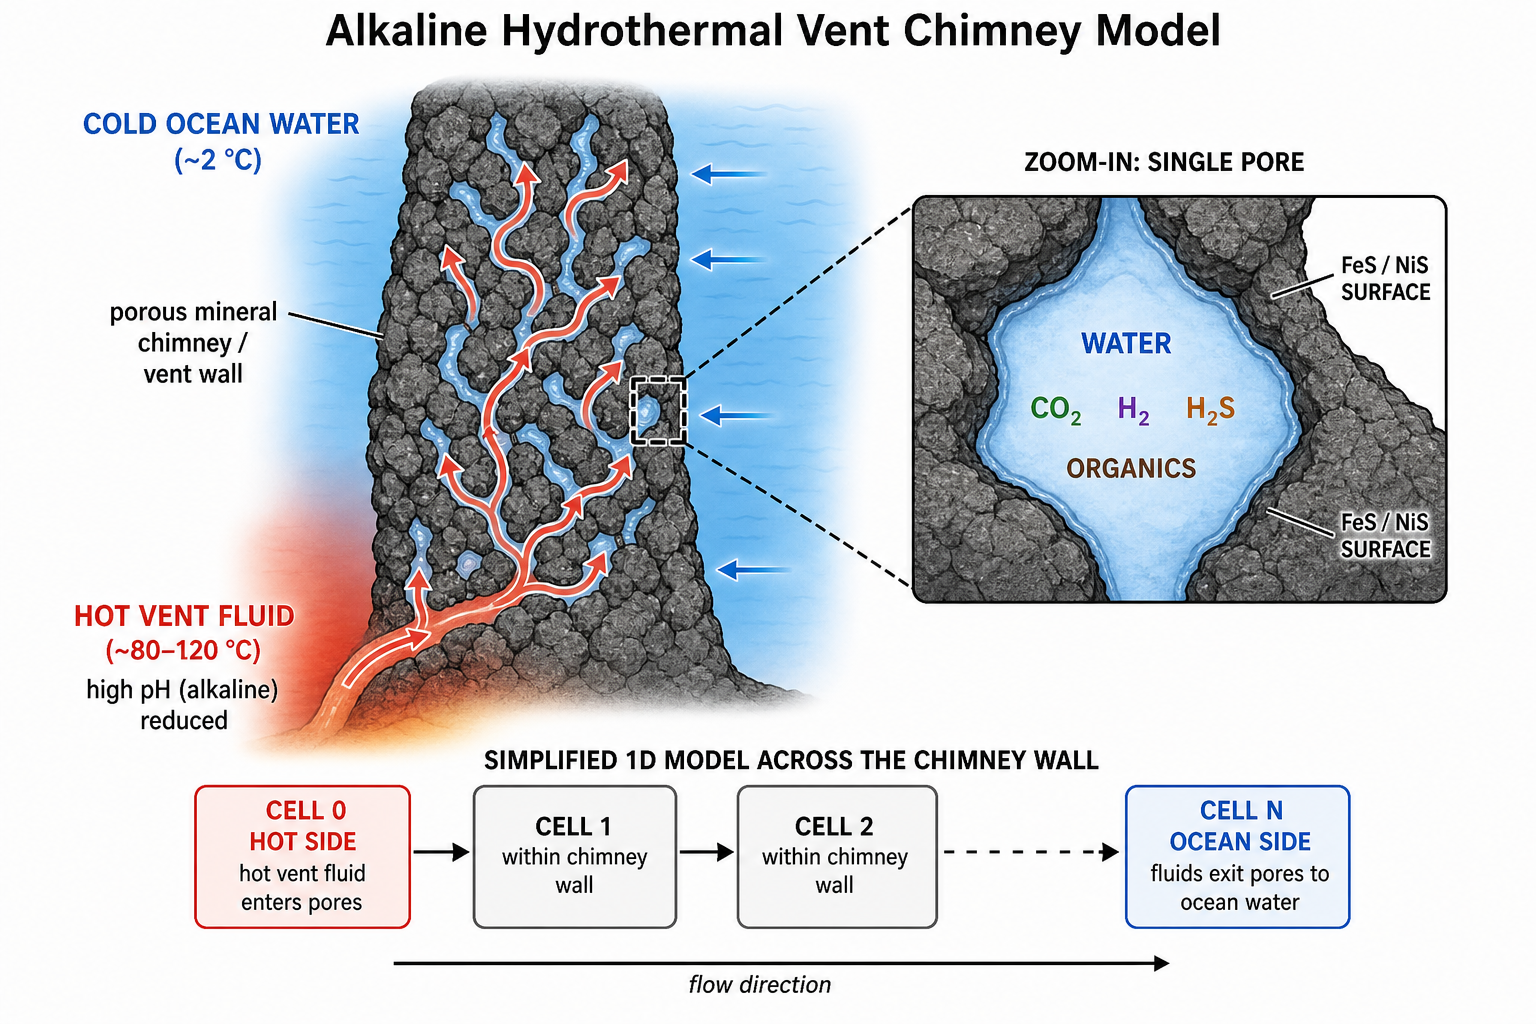
\includegraphics[width=0.95\linewidth]{hydrothermal_vent_chimney_model.png}
\caption{
Coarse-grained geometry of the hydrothermal vent model. The physical object is
a porous mineral chimney or vent wall separating hot reduced vent fluid from
colder ocean water. The one-dimensional coordinate is an effective coordinate
through this porous reactive wall, not an empty line in the ocean. Each model
cell represents a slice of water-filled mineral pores with local temperature,
pH, flow, dissolved chemistry, and reactive mineral surface area such as FeS
or NiS. Pore and surface chemistry happen first; coacervates and vesicle-like
objects are later products of that chemistry.
}
\end{figure}

\subsection{Top-level hydrothermal vent object}

The hydrothermal vent object represents a one-dimensional vent--ocean mixing
zone. It owns the environmental fields and the collection of compartment
objects living inside the vent system:
\begin{equation}
\mathcal{V}_{\rm vent}
=
\{
x_j,\ T_j,\ P_j,\ \mathrm{pH}_j,\ I_j,\ \mathrm{pe}_j,\ u_j,\ \lambda_j,
\mathbf{C}^{\rm env}_j,\ \mathbf{S}^{\rm mineral}_j,\ \mathcal{C}_j
\}.
\end{equation}
Here $x_j$ is the spatial coordinate, $u_j$ is the local flow velocity,
$\lambda_j$ is the vent/ocean mixing fraction, $\mathbf{C}^{\rm env}_j$ are
external aqueous concentrations or activities, $\mathbf{S}^{\rm mineral}_j$
stores reactive mineral surface availability, and $\mathcal{C}_j$ is the list
of compartments in cell $j$.

The main variables are:
\begin{itemize}
  \item $x_j$ is the position of cell $j$ across the porous chimney wall. The
  coordinate runs from hot vent side to cold ocean side.
  \item $T_j$ is the temperature in cell $j$.
  \item $P_j$ is the pressure in cell $j$.
  \item $\mathrm{pH}_j$ is the acidity/basicity in cell $j$.
  \item $I_j$ is ionic strength, a measure of dissolved salt content.
  \item $\mathrm{pe}_j$ is the redox state used by PHREEQC.
  \item $u_j$ is the effective flow velocity through the pores of cell $j$.
  \item $\lambda_j$ is the mixing fraction: $\lambda_j=1$ means pure vent
  fluid, $\lambda_j=0$ means pure ocean water.
  \item $\mathbf{C}^{\rm env}_j$ is the vector of dissolved external chemical
  concentrations in the pore water of cell $j$.
  \item $\mathbf{S}^{\rm mineral}_j$ stores available mineral surface area in
  cell $j$, for example FeS, NiS, magnetite, brucite, or silica surface.
  \item $\mathcal{C}_j$ is the list of compartments currently inside cell $j$,
  such as coacervates or vesicle candidates.
\end{itemize}

A first implementation can use fixed profiles:
\begin{align}
T(x) &= T_{\rm vent} + (T_{\rm ocean}-T_{\rm vent})x/L,\\
\lambda(x) &= \exp(-x/\ell_{\rm mix}),\\
C_i^{\rm env}(x) &= \lambda(x)C_{i,\rm vent} + [1-\lambda(x)]C_{i,\rm ocean}.
\end{align}
Later, these profiles can be replaced by advection--diffusion and PHREEQC
transport.

\subsection{Spatial cells}

Each spatial cell is a local reactor environment:
\begin{equation}
\mathcal{G}_j
=
\{
T_j,\ P_j,\ \mathrm{pH}_j,\ I_j,\ \mathrm{pe}_j,\ \mathbf{a}_j,\ 
\mathrm{SI}_{m,j},\ A_{m,j},\ u_j
\}.
\end{equation}
PHREEQC should provide the geochemical quantities $\mathbf{a}_j$,
$\mathrm{SI}_{m,j}$, and mineral constraints. The organic kinetic network then
uses these values to compute effective rates.

\subsection{Mineral pore reactors}

A pore is a fixed environmental compartment, not a protocell. It does not
divide and it is not inherited. It is the first hydrothermal object that can
concentrate and process chemistry.

For pore $k$ in spatial cell $j$:
\begin{equation}
\mathcal{P}_{jk}
=
\{
x_j,\ r_k,\ L_k,\ V_k,\ A_k,\ \mathbf{C}_{jk}^{\rm pore},
\mathbf{A}_{jk}^{\rm mineral},\ \tau_{jk}^{\rm res},\ q_{jk}
\}.
\end{equation}
The pore volume and surface area can initially be
\begin{align}
V_k &= \pi r_k^2 L_k,\\
A_k &= 2\pi r_k L_k,\\
\frac{A_k}{V_k} &= \frac{2}{r_k}.
\end{align}

The pore chemistry evolves as
\begin{equation}
\frac{dC_{i,k}^{\rm pore}}{dt}
=
\sum_\alpha \nu_{i\alpha} r_{\alpha,k}^{\rm pore}
+
k_{i,k}^{\rm in}C_{i,j}^{\rm env}
-
k_{i,k}^{\rm out}C_{i,k}^{\rm pore}
-
k_{i,k}^{\rm loss}C_{i,k}^{\rm pore}.
\end{equation}
The reaction rate inside a pore is
\begin{equation}
r_{\alpha,k}^{\rm pore}
=
k_{\alpha}(T_j)
\prod_i (C_{i,k}^{\rm pore})^{\nu_{i\alpha}^{+}}
f_\alpha(\mathrm{pH}_j)
g_\alpha(I_j)
h_\alpha(\mathbf{A}_{jk}^{\rm mineral})
q_\alpha(\mathrm{pe}_j).
\end{equation}

The residence-time interpretation is
\begin{equation}
k_{i,k}^{\rm out}\sim \frac{1}{\tau_{jk}^{\rm res}},
\qquad
\tau_{jk}^{\rm res}\sim \frac{L_k}{u_j}.
\end{equation}
Small pores have large surface-to-volume ratio and therefore stronger surface
chemistry, but high flow can flush products before autocatalytic or
compartment-forming chemistry accumulates.

\subsection{Surface-bound reaction domains}

Surface domains are reaction states attached to minerals rather than enclosed
volumes. They matter in hydrothermal vents because FeS, NiS, magnetite, brucite,
and silica can retain intermediates and catalyze carbonyl, thioester, peptide,
and redox chemistry.

For adsorbed species $i$ on mineral $m$:
\begin{equation}
\frac{d\Gamma_{i,m}}{dt}
=
k_{i,m}^{\rm ads}C_i^{\rm env}(1-\theta_m)
-
k_{i,m}^{\rm des}\Gamma_{i,m}
+
\sum_\alpha \nu_{i\alpha} r_{\alpha,m}^{\rm surf}
-
k_{i,m}^{\rm foul}\Gamma_{i,m}.
\end{equation}
Here $\Gamma_{i,m}$ is surface loading and $\theta_m$ is fractional site
coverage. Surface poisoning or refractory organic buildup should be represented
as loss of available mineral sites.

\subsection{Coacervate droplets as the first evolvable compartments}

A coacervate is not a protocell, but it is the first mobile compartment that can
carry a partially heritable internal composition. Coacervates form when the
pore/surface chemistry produces enough oppositely charged or mutually
phase-separating polymers, peptides, hetero-oligomers, or metal-organic
complexes.

In this model, a coacervate means a membrane-free, organic-rich liquid droplet
inside water. It is a dense liquid phase, not a lipid vesicle. The reason it is
important is that some molecules can become much more concentrated inside the
droplet than in the surrounding water. This concentration can make otherwise
slow reactions fast enough to matter.

Define a local coacervation score:
\begin{equation}
\Phi_{\rm coa}(j)
=
\sum_{a\in A}\sum_{b\in B}
\alpha_{ab}
C_{a,j}^{\rm env}
C_{b,j}^{\rm env}
f_{\rm pH}(\mathrm{pH}_j)
f_I(I_j).
\end{equation}

The symbols in this score mean:
\begin{itemize}
  \item $\Phi_{\rm coa}(j)$ is the tendency of spatial cell $j$ to form
  coacervate droplets.
  \item $j$ labels one slice of the one-dimensional porous vent wall.
  \item $A$ and $B$ are two classes of molecules that can phase-separate
  together, for example oppositely charged peptides or organic polymers.
  \item $C_{a,j}^{\rm env}$ is the concentration of molecule or pool $a$ in
  the external water of cell $j$.
  \item $C_{b,j}^{\rm env}$ is the concentration of molecule or pool $b$ in
  the same external water.
  \item $\alpha_{ab}$ measures how strongly species class $a$ and species
  class $b$ promote droplet formation.
  \item $f_{\rm pH}(\mathrm{pH}_j)$ reduces or enhances coacervation depending
  on the local pH.
  \item $f_I(I_j)$ reduces or enhances coacervation depending on ionic
  strength. High salt can screen charges and destabilize some coacervates.
\end{itemize}

Coacervate birth is allowed when
\begin{equation}
\Phi_{\rm coa}(j)>\Phi_{\rm coa}^{\rm crit}.
\end{equation}
Here $\Phi_{\rm coa}^{\rm crit}$ is the threshold above which the local mixture
is treated as able to phase-separate into droplets.

At birth, droplet $d$ samples its internal inventory from the local environment
with partition coefficients:
\begin{equation}
N_{i,d}(t_{\rm birth})
\sim
\mathrm{Poisson}
\left[
K_{i,d}^{\rm coa}
C_{i,j}^{\rm env}
V_d
N_A
\right].
\end{equation}

The symbols in the birth equation mean:
\begin{itemize}
  \item $N_{i,d}$ is the number of molecules of species $i$ inside droplet $d$.
  \item $t_{\rm birth}$ is the time at which the droplet forms.
  \item $K_{i,d}^{\rm coa}$ is the partition coefficient of species $i$ into
  droplet $d$. If $K_{i,d}^{\rm coa}>1$, the molecule is enriched inside the
  droplet. If $K_{i,d}^{\rm coa}<1$, it is excluded.
  \item $C_{i,j}^{\rm env}$ is the concentration of species $i$ in the
  surrounding water of cell $j$.
  \item $V_d$ is the droplet volume.
  \item $N_A$ is Avogadro's number, converting concentration times volume into
  expected molecule number.
  \item $\mathrm{Poisson}[\cdots]$ means the actual molecule count is randomly
  sampled around the expected count.
\end{itemize}

The coacervate internal dynamics are
\begin{equation}
\frac{dC_{i,d}^{\rm coa}}{dt}
=
\sum_\alpha \nu_{i\alpha} r_{\alpha,d}^{\rm coa}
+
\frac{
K_{i,d}^{\rm coa}C_{i,j}^{\rm env}
-
C_{i,d}^{\rm coa}
}{\tau_{i,d}^{\rm part}}
-
k_{i,d}^{\rm loss}C_{i,d}^{\rm coa}.
\end{equation}

The symbols in the coacervate dynamics equation mean:
\begin{itemize}
  \item $C_{i,d}^{\rm coa}$ is the concentration of species $i$ inside
  coacervate droplet $d$.
  \item $\nu_{i\alpha}$ is the stoichiometric change of species $i$ in reaction
  $\alpha$: positive if the reaction produces $i$, negative if it consumes $i$.
  \item $r_{\alpha,d}^{\rm coa}$ is the rate of reaction $\alpha$ inside
  droplet $d$.
  \item $K_{i,d}^{\rm coa}C_{i,j}^{\rm env}$ is the concentration that species
  $i$ would approach inside the droplet if partitioning reached equilibrium.
  \item $\tau_{i,d}^{\rm part}$ is the exchange or partitioning timescale. Large
  values mean slow exchange with the environment; small values mean fast
  equilibration.
  \item $k_{i,d}^{\rm loss}$ is the loss or degradation rate of species $i$
  inside droplet $d$.
\end{itemize}

The partition coefficients $K_i^{\rm coa}$ and exchange times
$\tau_i^{\rm part}$ are evolvable or sampled traits in later simulations.

\subsection{Coacervate to vesicle transition}

The vesicle/protocell stage should be created by amphiphile accumulation, not
assumed at initialization. Track amphiphile coverage on the coacervate
interface:
\begin{equation}
\frac{dN_{L,d}}{dt}
=
k_{\rm ads}A_d C_{L,j}^{\rm env}
-
k_{\rm des}N_{L,d}
+
R_{L,d}^{\rm internal}.
\end{equation}
The required number of amphiphiles for a membrane-like coating is
\begin{equation}
N_{L,d}^{\rm req}
\approx
\frac{8\pi R_d^2}{a_L},
\end{equation}
where $a_L$ is the molecular area per amphiphile. Define coverage
\begin{equation}
\theta_d=\frac{N_{L,d}}{N_{L,d}^{\rm req}}.
\end{equation}
When
\begin{equation}
\theta_d \geq \theta_{\rm ves},
\end{equation}
the transition is
\begin{equation}
\text{coacervate droplet}
\rightarrow
\text{amphiphile-stabilized vesicle/protocell candidate}.
\end{equation}

\subsection{Lineage evolution should begin at the coacervate stage}

For hydrothermal vents, selection should not start from fully formed
protocells. The first selectable objects are coacervates or amphiphile-stabilized
droplets that persist, concentrate feedstocks, and enhance productive chemistry.
Their evolvable traits can be represented as
\begin{equation}
\Theta_d
=
\{
K_i^{\rm coa},\ \tau_i^{\rm part},\ 
\chi_{\rm eff},\ P_i,\ 
\mathcal{K}_{d\alpha}^{\rm cat},\ 
\theta_{\rm div}
\}.
\end{equation}
Here $\mathcal{K}_{d\alpha}^{\rm cat}$ is the droplet's catalytic enhancement
profile over the reference reaction network. Mutation changes these traits
between parent and daughter droplets.

An operational fitness for early hydrothermal compartment evolution is
\begin{equation}
F_d
=
w_R R_{\rm productive}
+
w_A A_{\rm autocatalytic}
+
w_E C_{\rm energy}
+
w_L C_{\rm amphiphile}
+
w_S t_{\rm survival}
-
w_D D_{\rm dilution}
-
w_H H_{\rm hydrolysis}
-
w_F F_{\rm fouling}.
\end{equation}
The first computational target is not ``life''. It is persistent,
compartmentalized, autocatalytic chemistry that can transition from mineral
pore/surface concentration into coacervate or vesicle-like objects.

\subsection{Minimal code objects}

The corresponding first implementation should expose these objects:
\begin{verbatim}
HydrothermalVent
    spatial_cells: list[VentCell]
    pore_compartments: list[PoreCompartment]
    coacervates: list[CoacervateDroplet]
    vesicles: list[VesicleCandidate]

VentCell
    x, T, P, pH, ionic_strength, pe, flow_velocity
    env_concentrations
    mineral_surfaces

PoreCompartment
    cell_id, radius, length, volume, surface_area
    mineral_surface_area
    concentrations
    residence_time

CoacervateDroplet
    cell_id, radius, volume
    internal_counts
    partition_coefficients
    partition_times
    catalytic_profile

VesicleCandidate
    cell_id, radius, volume, area
    internal_counts
    amphiphile_count
    permeability
\end{verbatim}

The hydrothermal vent branch should therefore implement chemistry in this order:
\begin{enumerate}
  \item parse the hydrothermal reference reaction network;
  \item build environmental feedstock and mineral-surface fields;
  \item run pore/surface chemistry;
  \item allow coacervate birth from enriched polymer/charged-organic pools;
  \item evolve coacervate internal chemistry and partitioning traits;
  \item convert successful droplets into vesicle/protocell candidates.
\end{enumerate}

\section{Initial conditions for water worlds}

The following numbers are not final observational constraints. They are scenario templates
for simulation design. Europa and Ganymede ocean compositions are uncertain; published
models commonly explore chloride-rich, sulfate-rich, carbonate-bearing, and water--rock
alteration scenarios \cite{tan2021,thompson2021,nasaEuropa2016,gavinVance2012}. The values
below should therefore be treated as tunable hypotheses.

\subsection{Scenario A: Europa-like oxidant-influenced chloride/sulfate ocean}

\begin{longtable}{lll}
\toprule
Quantity & Symbol & Starting value / range \\
\midrule
Ocean temperature & $T_{\rm ocean}$ & \SIrange{260}{290}{K} \\
Vent temperature & $T_{\rm vent}$ & \SIrange{320}{500}{K} \\
Seafloor pressure & $P_{\rm sf}$ & \SIrange{50}{150}{MPa} \\
pH initial guess & pH & 5.5--9.5 \\
Na & Na & 0.05--0.70 mol/kgw \\
Cl & Cl & 0.05--0.70 mol/kgw \\
Mg & Mg & $10^{-3}$--0.1 mol/kgw \\
Ca & Ca & $10^{-4}$--0.05 mol/kgw \\
Total carbonate & C(4) & $10^{-4}$--$10^{-1}$ mol/kgw \\
Sulfate & S(6) & $10^{-5}$--$10^{-1}$ mol/kgw \\
Sulfide & S(-2) & $10^{-8}$--$10^{-3}$ mol/kgw \\
Fe & Fe(2) & $10^{-9}$--$10^{-4}$ mol/kgw \\
Ni & Ni(2) & $10^{-10}$--$10^{-6}$ mol/kgw \\
Ammonia/ammonium & N(-3) & $10^{-8}$--$10^{-4}$ mol/kgw \\
Phosphate & P & $10^{-9}$--$10^{-5}$ mol/kgw \\
Silica & Si & $10^{-5}$--$10^{-2}$ mol/kgw \\
Hydrogen & H2(aq) & $10^{-8}$--$10^{-2}$ mol/kgw \\
Methane & CH4(aq) & $10^{-9}$--$10^{-3}$ mol/kgw \\
\bottomrule
\end{longtable}

\subsection{Scenario B: Ganymede-like more reduced ocean}

\begin{longtable}{lll}
\toprule
Quantity & Symbol & Starting value / range \\
\midrule
Ocean temperature & $T_{\rm ocean}$ & \SIrange{250}{290}{K} \\
Vent temperature & $T_{\rm vent}$ & \SIrange{310}{450}{K} \\
Seafloor pressure & $P_{\rm sf}$ & \SIrange{80}{250}{MPa} \\
pH initial guess & pH & 7.0--11.5 \\
Na & Na & 0.01--0.50 mol/kgw \\
Cl & Cl & 0.01--0.50 mol/kgw \\
Mg & Mg & $10^{-4}$--0.05 mol/kgw \\
Ca & Ca & $10^{-5}$--0.02 mol/kgw \\
Total carbonate & C(4) & $10^{-5}$--$10^{-1}$ mol/kgw \\
Sulfate & S(6) & $10^{-8}$--$10^{-3}$ mol/kgw \\
Sulfide & S(-2) & $10^{-7}$--$10^{-2}$ mol/kgw \\
Fe & Fe(2) & $10^{-9}$--$10^{-4}$ mol/kgw \\
Ni & Ni(2) & $10^{-10}$--$10^{-6}$ mol/kgw \\
Ammonia/ammonium & N(-3) & $10^{-8}$--$10^{-4}$ mol/kgw \\
Phosphate & P & $10^{-10}$--$10^{-5}$ mol/kgw \\
Silica & Si & $10^{-5}$--$10^{-2}$ mol/kgw \\
Hydrogen & H2(aq) & $10^{-7}$--$10^{-2}$ mol/kgw \\
Methane & CH4(aq) & $10^{-8}$--$10^{-3}$ mol/kgw \\
\bottomrule
\end{longtable}

\subsection{Scenario C: generic Enceladus-like alkaline hydrothermal ocean}

This case is useful as a positive-control scenario for alkaline hydrothermal chemistry.
\begin{longtable}{lll}
\toprule
Quantity & Symbol & Starting value / range \\
\midrule
Ocean temperature & $T_{\rm ocean}$ & \SIrange{270}{300}{K} \\
Vent temperature & $T_{\rm vent}$ & \SIrange{330}{500}{K} \\
Seafloor pressure & $P_{\rm sf}$ & \SIrange{5}{50}{MPa} \\
pH initial guess & pH & 8.5--12.0 \\
Na & Na & 0.05--0.80 mol/kgw \\
Cl & Cl & 0.05--0.80 mol/kgw \\
Carbonate & C(4) & $10^{-4}$--$10^{-1}$ mol/kgw \\
Sulfide & S(-2) & $10^{-7}$--$10^{-2}$ mol/kgw \\
Hydrogen & H2(aq) & $10^{-6}$--$10^{-1}$ mol/kgw \\
Methane & CH4(aq) & $10^{-8}$--$10^{-2}$ mol/kgw \\
Silica & Si & $10^{-5}$--$10^{-2}$ mol/kgw \\
\bottomrule
\end{longtable}

\section{PHREEQC input templates}

\subsection{Ocean boundary template}

\begin{verbatim}
TITLE Europa-like ocean boundary
SOLUTION 1 Ocean
    temp      {T_ocean_C}
    pressure  {P_ocean_atm}
    units     mol/kgw
    pH        {pH_guess} charge
    pe        {pe_guess}
    Na        {Na}
    Cl        {Cl}
    Mg        {Mg}
    Ca        {Ca}
    C(4)      {C_total}
    S(6)      {Sulfate}
    S(-2)     {Sulfide}
    Fe(2)     {Fe2}
    Ni        {Ni2}
    N(-3)     {NH3_total}
    P         {P_total}
    Si        {Si_total}
    H(0)      {H2_total}
END
\end{verbatim}

\subsection{Vent boundary template}

\begin{verbatim}
TITLE Reduced hydrothermal vent boundary
SOLUTION 2 Vent
    temp      {T_vent_C}
    pressure  {P_vent_atm}
    units     mol/kgw
    pH        {pH_vent_guess} charge
    pe        {pe_vent_guess}
    Na        {Na_vent}
    Cl        {Cl_vent}
    Mg        {Mg_vent}
    Ca        {Ca_vent}
    C(4)      {C_vent}
    S(-2)     {Sulfide_vent}
    Fe(2)     {Fe2_vent}
    Ni        {Ni2_vent}
    N(-3)     {NH3_vent}
    P         {P_vent}
    Si        {Si_vent}
    H(0)      {H2_vent}
EQUILIBRIUM_PHASES
    Mackinawite  0.0  0.0
    Pyrite       0.0  0.0
    Magnetite    0.0  0.0
    Brucite      0.0  0.0
    Calcite      0.0  0.0
END
\end{verbatim}

\section{PHREEQC outputs required by the kinetic network}

At each grid cell, extract:
\begin{longtable}{lll}
\toprule
Output & Symbol & Use in kinetic network \\
\midrule
pH & $\mathrm{pH}$ & Acid/base control, vesicle stability \\
pe/Eh & $\mathrm{pe}$ or $E_h$ & Redox availability \\
Ionic strength & $I$ & Activity corrections, vesicle stress \\
\ch{CO2(aq)} & $a_{\ch{CO2}}$ & Carbon fixation \\
\ch{HCO3-} & $a_{\ch{HCO3-}}$ & Carbonate buffer, carbon source \\
\ch{CO3^{2-}} & $a_{\ch{CO3^{2-}}}$ & Carbonate precipitation \\
\ch{H2(aq)} & $a_{\ch{H2}}$ & Electron donor \\
\ch{CO(aq)} & $a_{\ch{CO}}$ & Carbonyl chemistry \\
\ch{H2S}, \ch{HS-} & $a_{\rm sulfide}$ & FeS formation, thioester chemistry \\
\ch{Fe^{2+}}, \ch{Ni^{2+}} & $a_{\rm Fe}, a_{\rm Ni}$ & Catalytic mineral availability \\
\ch{NH3}, \ch{NH4+} & $a_{\rm N}$ & Amino acid precursors \\
Phosphate species & $a_{\rm Pi}$ & Acetyl phosphate, activation chemistry \\
\ch{Mg^{2+}}, \ch{Ca^{2+}} & $a_{\rm Mg},a_{\rm Ca}$ & Fatty acid precipitation/stability \\
Mineral SI & $\mathrm{SI}_m$ & Surface availability and precipitation sinks \\
\bottomrule
\end{longtable}

\section{Reaction network}

The following reaction network is deliberately written as an implementable starting model.
Some reactions are elementary-looking; others are lumped effective reactions representing
families of pathways. Each reaction should carry a confidence flag and a literature source
in the code.

\subsection{Module A: aqueous acid--base and geochemical equilibria}

These reactions should mostly be handled by PHREEQC, not by the custom kinetic layer.

\begin{longtable}{p{0.08\linewidth}p{0.70\linewidth}p{0.18\linewidth}}
\toprule
ID & Reaction & Role \\
\midrule
G1 & \ch{CO2(aq) + H2O <=> HCO3- + H+} & carbonate speciation \\
G2 & \ch{HCO3- <=> CO3^{2-} + H+} & carbonate speciation \\
G3 & \ch{H2S <=> HS- + H+} & sulfide speciation \\
G4 & \ch{HS- <=> S^{2-} + H+} & sulfide speciation \\
G5 & \ch{NH4+ <=> NH3 + H+} & nitrogen speciation \\
G6 & \ch{H3PO4 <=> H2PO4- + H+} & phosphate speciation \\
G7 & \ch{H2PO4- <=> HPO4^{2-} + H+} & phosphate speciation \\
G8 & \ch{HPO4^{2-} <=> PO4^{3-} + H+} & phosphate speciation \\
G9 & \ch{Fe^{2+} + HS- -> FeS(s) + H+} & FeS precipitation \\
G10 & \ch{Ni^{2+} + HS- -> NiS(s) + H+} & NiS precipitation \\
G11 & \ch{Ca^{2+} + CO3^{2-} -> CaCO3(s)} & carbonate sink \\
G12 & \ch{Mg^{2+} + 2OH- -> Mg(OH)2(s)} & brucite sink \\
G13 & \ch{3Fe^{2+} + 4H2O -> Fe3O4(s) + 8H+ + 2e-} & magnetite/redox \\
G14 & \ch{FeS(s) + S^0 -> FeS2(s)} & pyrite formation \\
G15 & \ch{SiO2(aq) -> SiO2(s)} & silica precipitation \\
\bottomrule
\end{longtable}

\subsection{Module B: C1 carbon fixation and redox entry}

\begin{longtable}{p{0.08\linewidth}p{0.70\linewidth}p{0.18\linewidth}}
\toprule
ID & Reaction & Catalyst / control \\
\midrule
R1 & \ch{CO2 + H2 -> HCOO- + H+} & FeS/NiS/magnetite \\
R2 & \ch{CO2 + H2 -> CO + H2O} & Fe/Ni minerals \\
R3 & \ch{CO + H2O -> CO2 + H2} & water--gas shift \\
R4 & \ch{CO2 + 4H2 -> CH4 + 2H2O} & methanation sink \\
R5 & \ch{HCOO- + H+ <=> HCOOH} & PHREEQC/pH \\
R6 & \ch{CO2 + HS- + H+ -> COS + H2O} & sulfide activation \\
R7 & \ch{COS + H2O -> CO2 + H2S} & hydrolysis sink \\
R8 & \ch{COS + NH3 -> NH2CO-SH} & carbamoyl/thiocarbamate pool \\
R9 & \ch{CO + H2S -> COS + H2} & sulfur-carbonyl pool \\
R10 & \ch{HCOO- + H2 -> HCHO + OH-} & reduced C1 pool \\
\bottomrule
\end{longtable}

\subsection{Module C: thioester and acetyl-phosphate activation}

\begin{longtable}{p{0.08\linewidth}p{0.70\linewidth}p{0.18\linewidth}}
\toprule
ID & Reaction & Catalyst / control \\
\midrule
R11 & \ch{CO + CH3SH -> CH3COSR} & FeS/NiS surface \\
R12 & \ch{CO2 + CH3SH + 2H2 -> CH3COSR + 2H2O} & Fe/Ni sulfides \\
R13 & \ch{CH3COSR + H2O -> CH3COO- + RSH + H+} & hydrolysis sink \\
R14 & \ch{CH3COSR + Pi -> CH3COOPO3^{2-} + RSH} & acetyl phosphate \\
R15 & \ch{CH3COOPO3^{2-} + H2O -> CH3COO- + Pi + H+} & hydrolysis sink \\
R16 & \ch{CH3COOPO3^{2-} + NH3 -> acetamide + Pi} & amide side branch \\
R17 & \ch{CH3COSR + NH3 -> thioacetamide + RSH} & nitrogen side branch \\
R18 & \ch{CH3COSR + HCOO- -> acetoacetyl\_SR} & C--C extension \\
R19 & \ch{CH3COSR + CO2 + H2 -> pyruvate + RSH} & C3 precursor \\
R20 & \ch{CH3COO- + H+ <=> CH3COOH} & PHREEQC/pH \\
\bottomrule
\end{longtable}

\subsection{Module D: C2--C5 central organic precursor network}

\begin{longtable}{p{0.08\linewidth}p{0.70\linewidth}p{0.18\linewidth}}
\toprule
ID & Reaction & Catalyst / control \\
\midrule
R21 & \ch{HCHO + HCHO -> glycolaldehyde} & mineral/base catalysis \\
R22 & \ch{glycolaldehyde + HCHO -> glyceraldehyde} & sugar precursor \\
R23 & \ch{glycolaldehyde + HCN -> glycolonitrile} & nitrile branch \\
R24 & \ch{HCHO + HCN -> glycolonitrile} & nitrile branch \\
R25 & \ch{glycolonitrile + 2H2O -> glycolate + NH3} & hydrolysis \\
R26 & \ch{acetate + CO2 + H2 -> pyruvate + H2O} & Fe/Ni minerals \\
R27 & \ch{pyruvate + CO2 + H2 -> oxaloacetate} & C4 precursor \\
R28 & \ch{pyruvate + H2 -> lactate} & reduction sink \\
R29 & \ch{pyruvate -> acetate + CO2} & decarboxylation sink \\
R30 & \ch{glyoxylate + acetate -> malate} & C4 pool abstraction \\
R31 & \ch{malate -> fumarate + H2O} & dehydration \\
R32 & \ch{fumarate + H2 -> succinate} & reduction \\
R33 & \ch{succinate + CO2 + H2 -> alpha\mbox{-}ketoglutarate} & C5 precursor \\
R34 & \ch{alpha\mbox{-}ketoglutarate -> succinate + CO2} & degradation sink \\
R35 & \ch{oxaloacetate -> pyruvate + CO2} & degradation sink \\
\bottomrule
\end{longtable}

\subsection{Module E: amino-acid precursor network}

\begin{longtable}{p{0.08\linewidth}p{0.70\linewidth}p{0.18\linewidth}}
\toprule
ID & Reaction & Catalyst / control \\
\midrule
R36 & \ch{glyoxylate + NH3 + H2 -> glycine + H2O} & reductive amination \\
R37 & \ch{pyruvate + NH3 + H2 -> alanine + H2O} & reductive amination \\
R38 & \ch{oxaloacetate + NH3 + H2 -> aspartate + H2O} & reductive amination \\
R39 & \ch{alpha\mbox{-}ketoglutarate + NH3 + H2 -> glutamate + H2O} & reductive amination \\
R40 & \ch{HCHO + NH3 + HCN -> aminoacetonitrile + H2O} & Strecker-like \\
R41 & \ch{aminoacetonitrile + 2H2O -> glycine + NH3} & hydrolysis \\
R42 & \ch{acetaldehyde + NH3 + HCN -> alanine\_nitrile + H2O} & Strecker-like \\
R43 & \ch{alanine\_nitrile + 2H2O -> alanine + NH3} & hydrolysis \\
R44 & \ch{amino\_acid + H2O -> degradation\_products} & hydrolysis/degradation \\
R45 & \ch{amino\_acid + mineral -> amino\_acid\_surface} & retention \\
\bottomrule
\end{longtable}

\subsection{Module F: peptide and activated condensation network}

\begin{longtable}{p{0.08\linewidth}p{0.70\linewidth}p{0.18\linewidth}}
\toprule
ID & Reaction & Catalyst / control \\
\midrule
R46 & \ch{AA + acetylP -> AA^* + acetate} & activation \\
R47 & \ch{AA^* + AA -> peptide2 + Pi} & condensation \\
R48 & \ch{peptide_n + AA^* -> peptide_{n+1} + Pi} & chain growth \\
R49 & \ch{peptide_n + H2O -> peptide_{n-1} + AA} & hydrolysis \\
R50 & \ch{peptide_n + mineral -> peptide_n\_surface} & retention/catalysis \\
R51 & \ch{peptide\_surface + FA -> peptide\_FA\_complex} & membrane stabilization \\
R52 & \ch{AA^* + H2O -> AA + Pi} & activation loss \\
R53 & \ch{peptide_n -> degraded\_organic\_pool} & thermal degradation \\
\bottomrule
\end{longtable}

\subsection{Module G: fatty-acid, amphiphile, and vesicle network}

\begin{longtable}{p{0.08\linewidth}p{0.70\linewidth}p{0.18\linewidth}}
\toprule
ID & Reaction & Catalyst / control \\
\midrule
R54 & \ch{CO + H2 -> CH2^* + H2O} & Fischer--Tropsch-like \\
R55 & \ch{CH2^* + acyl\_C_n -> acyl\_C_{n+1}} & chain growth \\
R56 & \ch{acetyl\mbox{-}SR + CH2^* -> acyl\_C3\mbox{-}SR} & chain initiation \\
R57 & \ch{acyl\_C_n\mbox{-}SR + H2O -> FA\_C_n + RSH} & fatty acid release \\
R58 & \ch{FA\_C_n + Mg^{2+} -> Mg(FA)_2(s)} & precipitation sink \\
R59 & \ch{FA\_C_n + Ca^{2+} -> Ca(FA)_2(s)} & precipitation sink \\
R60 & \ch{FA\_C_n + H+ <=> HFA\_C_n} & pH-dependent protonation \\
R61 & \ch{FA\_C_n -> micelle} & self-assembly \\
R62 & \ch{micelle + FA\_C_n -> vesicle} & growth \\
R63 & \ch{vesicle + FA\_C_n -> larger\_vesicle} & membrane growth \\
R64 & \ch{vesicle + peptide -> stabilized\_vesicle} & stabilization \\
R65 & \ch{vesicle -> micelle + FA\_loss} & disruption \\
R66 & \ch{stabilized\_vesicle + organics -> protocell\_candidate} & protocell nucleation \\
\bottomrule
\end{longtable}

\section{Rate-law templates}

For each reaction $\alpha$, store:
\begin{verbatim}
{
  "id": "R1",
  "reactants": {"CO2": 1, "H2": 1},
  "products": {"formate": 1, "H+": 1},
  "phase": "surface_aqueous",
  "catalysts": ["FeS", "NiS", "magnetite"],
  "k0": null,
  "Ea_kJ_mol": null,
  "pH_window": [8.0, 11.5],
  "T_window_K": [273, 500],
  "depends_on_phreeqc": ["CO2", "H2", "pH", "pe", "FeS_SI", "NiS_SI"],
  "confidence": "medium",
  "reference": ["MartinRussell2006", "Sojo2016"]
}
\end{verbatim}

Use activities where possible:
\begin{equation}
r_{\ch{CO2}\rightarrow \ch{formate}}
=
k_1(T)
a_{\ch{CO2}}
a_{\ch{H2}}
h_{\rm FeS/NiS}
f_{\rm pH}
f_{\rm redox}.
\end{equation}

For fatty-acid vesicle formation:
\begin{equation}
r_{\rm ves}
=
k_{\rm ves}
C_{\rm FA}
f_{\rm pH}(\mathrm{pH})
f_I(I)
f_{\rm div}(a_{\ch{Mg^{2+}}},a_{\ch{Ca^{2+}}}),
\end{equation}
with $f_{\rm div}$ decreasing when divalent cations precipitate fatty acids.

\section{Numerical algorithm}

\begin{enumerate}
\item Build planet object and compute $T(x)$, $P(x)$, flow velocity $u(x)$, and energy/redox fluxes.
\item Initialize bulk element totals for ocean and vent endmembers.
\item For each grid cell, mix ocean and vent endmembers:
\begin{equation}
b_i(x)=\lambda(x)b_i^{\rm vent}+[1-\lambda(x)]b_i^{\rm ocean}.
\end{equation}
\item Run PHREEQC at each grid cell using $T(x)$, $P(x)$, $b_i(x)$, gas constraints, and mineral phases.
\item Extract $\mathrm{pH}$, $\mathrm{pe}$, ionic strength, activities, and mineral saturation indices.
\item Evaluate kinetic rates $r_\alpha$ for the organic network using PHREEQC output.
\item Update organic concentrations by reaction--transport.
\item Feed selected organic totals back into PHREEQC only if they significantly affect charge balance, complexation, or precipitation.
\item Compute local protocell nucleation probability.
\item Create, evolve, divide, or destroy protocell agents.
\end{enumerate}

\section{Python object interfaces}

\subsection{Planet state}

\begin{verbatim}
@dataclass
class PlanetState:
    name: str
    radius_m: float
    mass_kg: float
    gravity_m_s2: float
    ocean_depth_m: float
    ice_shell_thickness_m: float
    tidal_heat_flux_W_m2: float
    radiogenic_heat_flux_W_m2: float
    oxidant_flux_mol_m2_s: float
    rock_model: str
\end{verbatim}

\subsection{Geochemical cell input}

\begin{verbatim}
@dataclass
class GeoCellInput:
    T_K: float
    P_Pa: float
    totals_mol_kgw: dict
    pH_guess: float
    pe_guess: float
    minerals: list
    gases: dict
\end{verbatim}

\subsection{PHREEQC output state}

\begin{verbatim}
@dataclass
class GeoState:
    pH: float
    pe: float
    ionic_strength: float
    activities: dict
    concentrations: dict
    saturation_indices: dict
    mineral_amounts: dict
\end{verbatim}

\subsection{Organic network state}

\begin{verbatim}
@dataclass
class OrganicState:
    formate: float
    formaldehyde: float
    CO: float
    acetate: float
    pyruvate: float
    oxaloacetate: float
    acetyl_thioester: float
    acetyl_phosphate: float
    amino_acid_pool: float
    activated_amino_acid_pool: float
    peptide_pool: float
    fatty_acid_pool: float
    micelle_pool: float
    vesicle_pool: float
\end{verbatim}

\subsection{Protocell agent}

\begin{verbatim}
@dataclass
class Protocell:
    position: float
    lipid_inventory: float
    peptide_inventory: float
    energy_inventory: float
    permeability: float
    stability: float
    catalyst_genotype: dict
    size: float
    age: float
\end{verbatim}

\section{References}

\begin{thebibliography}{99}

\bibitem{parkhurst1995}
D. L. Parkhurst,
\emph{User's guide to PHREEQC: A computer program for speciation, reaction-path,
advective-transport, and inverse geochemical calculations},
U.S. Geological Survey Water-Resources Investigations Report 95-4227, 1995.
\url{https://pubs.usgs.gov/publication/wri954227}

\bibitem{parkhurst1999}
D. L. Parkhurst and C. A. J. Appelo,
\emph{User's guide to PHREEQC (Version 2): A computer program for speciation,
batch-reaction, one-dimensional transport, and inverse geochemical calculations},
U.S. Geological Survey Water-Resources Investigations Report 99-4259, 1999.
\url{https://pubs.usgs.gov/publication/wri994259}

\bibitem{parkhurst2013}
D. L. Parkhurst and C. A. J. Appelo,
\emph{Description of input and examples for PHREEQC version 3},
U.S. Geological Survey Techniques and Methods, 2013.
\url{https://water.usgs.gov/water-resources/software/PHREEQC/}

\bibitem{martinRussell2006}
W. Martin and M. J. Russell,
On the origin of biochemistry at an alkaline hydrothermal vent,
\emph{Philosophical Transactions of the Royal Society B}, 2007.
\url{https://pmc.ncbi.nlm.nih.gov/articles/PMC2442388/}

\bibitem{sojo2016}
V. Sojo, B. Herschy, A. Whicher, E. Camprubi, and N. Lane,
The origin of life in alkaline hydrothermal vents,
\emph{Astrobiology}, 2016.
\url{https://pubmed.ncbi.nlm.nih.gov/26841066/}

\bibitem{whicher2018}
A. Whicher et al.,
Acetyl phosphate as a primordial energy currency at the origin of life,
\emph{Origins of Life and Evolution of Biospheres}, 2018.
\url{https://pmc.ncbi.nlm.nih.gov/articles/PMC6061221/}

\bibitem{tan2021}
S. Tan et al.,
Laboratory experiments on sulfate reduction at 100 MPa: Implications for Europa's ocean,
\emph{Icarus}, 2021.
\url{https://www.sciencedirect.com/science/article/abs/pii/S0019103520305522}

\bibitem{thompson2021}
S. P. Thompson et al.,
Laboratory exploration of mineral precipitates from Europa's ocean composition analogs,
2021.
\url{https://pmc.ncbi.nlm.nih.gov/articles/PMC8493616/}

\bibitem{nasaEuropa2016}
NASA,
Europa's ocean may have an Earthlike chemical balance, 2016.
\url{https://science.nasa.gov/missions/europa-clipper/europas-ocean-may-have-an-earthlike-chemical-balance/}

\bibitem{gavinVance2012}
P. Gavin and S. Vance,
Modeling hydrothermal vents on Europa,
Lunar and Planetary Science Conference, 2012.
\url{https://www.lpi.usra.edu/meetings/lpsc2012/pdf/1683.pdf}

\end{thebibliography}

\end{document}
